\documentclass[twoside]{book}

% Packages required by doxygen
\usepackage{fixltx2e}
\usepackage{calc}
\usepackage{doxygen}
\usepackage[export]{adjustbox} % also loads graphicx
\usepackage{graphicx}
\usepackage[utf8]{inputenc}
\usepackage{makeidx}
\usepackage{multicol}
\usepackage{multirow}
\PassOptionsToPackage{warn}{textcomp}
\usepackage{textcomp}
\usepackage[nointegrals]{wasysym}
\usepackage[table]{xcolor}

% Font selection
\usepackage[T1]{fontenc}
\usepackage[scaled=.90]{helvet}
\usepackage{courier}
\usepackage{amssymb}
\usepackage{sectsty}
\renewcommand{\familydefault}{\sfdefault}
\allsectionsfont{%
  \fontseries{bc}\selectfont%
  \color{darkgray}%
}
\renewcommand{\DoxyLabelFont}{%
  \fontseries{bc}\selectfont%
  \color{darkgray}%
}
\newcommand{\+}{\discretionary{\mbox{\scriptsize$\hookleftarrow$}}{}{}}

% Page & text layout
\usepackage{geometry}
\geometry{%
  a4paper,%
  top=2.5cm,%
  bottom=2.5cm,%
  left=2.5cm,%
  right=2.5cm%
}
\tolerance=750
\hfuzz=15pt
\hbadness=750
\setlength{\emergencystretch}{15pt}
\setlength{\parindent}{0cm}
\setlength{\parskip}{3ex plus 2ex minus 2ex}
\makeatletter
\renewcommand{\paragraph}{%
  \@startsection{paragraph}{4}{0ex}{-1.0ex}{1.0ex}{%
    \normalfont\normalsize\bfseries\SS@parafont%
  }%
}
\renewcommand{\subparagraph}{%
  \@startsection{subparagraph}{5}{0ex}{-1.0ex}{1.0ex}{%
    \normalfont\normalsize\bfseries\SS@subparafont%
  }%
}
\makeatother

% Headers & footers
\usepackage{fancyhdr}
\pagestyle{fancyplain}
\fancyhead[LE]{\fancyplain{}{\bfseries\thepage}}
\fancyhead[CE]{\fancyplain{}{}}
\fancyhead[RE]{\fancyplain{}{\bfseries\leftmark}}
\fancyhead[LO]{\fancyplain{}{\bfseries\rightmark}}
\fancyhead[CO]{\fancyplain{}{}}
\fancyhead[RO]{\fancyplain{}{\bfseries\thepage}}
\fancyfoot[LE]{\fancyplain{}{}}
\fancyfoot[CE]{\fancyplain{}{}}
\fancyfoot[RE]{\fancyplain{}{\bfseries\scriptsize Generated by Doxygen }}
\fancyfoot[LO]{\fancyplain{}{\bfseries\scriptsize Generated by Doxygen }}
\fancyfoot[CO]{\fancyplain{}{}}
\fancyfoot[RO]{\fancyplain{}{}}
\renewcommand{\footrulewidth}{0.4pt}
\renewcommand{\chaptermark}[1]{%
  \markboth{#1}{}%
}
\renewcommand{\sectionmark}[1]{%
  \markright{\thesection\ #1}%
}

% Indices & bibliography
\usepackage{natbib}
\usepackage[titles]{tocloft}
\setcounter{tocdepth}{3}
\setcounter{secnumdepth}{5}
\makeindex

% Hyperlinks (required, but should be loaded last)
\usepackage{ifpdf}
\ifpdf
  \usepackage[pdftex,pagebackref=true]{hyperref}
\else
  \usepackage[ps2pdf,pagebackref=true]{hyperref}
\fi
\hypersetup{%
  colorlinks=true,%
  linkcolor=blue,%
  citecolor=blue,%
  unicode%
}

% Custom commands
\newcommand{\clearemptydoublepage}{%
  \newpage{\pagestyle{empty}\cleardoublepage}%
}

\usepackage{caption}
\captionsetup{labelsep=space,justification=centering,font={bf},singlelinecheck=off,skip=4pt,position=top}

%===== C O N T E N T S =====

\begin{document}

% Titlepage & ToC
\hypersetup{pageanchor=false,
             bookmarksnumbered=true,
             pdfencoding=unicode
            }
\pagenumbering{alph}
\begin{titlepage}
\vspace*{7cm}
\begin{center}%
{\Large M\+RR Turnouts }\\
\vspace*{1cm}
{\large Generated by Doxygen 1.8.13}\\
\end{center}
\end{titlepage}
\clearemptydoublepage
\pagenumbering{roman}
\tableofcontents
\clearemptydoublepage
\pagenumbering{arabic}
\hypersetup{pageanchor=true}

%--- Begin generated contents ---
\chapter{Q\+T5 Turnout control using M\+Q\+TT and a Raspberry Pi}
\label{index}\hypertarget{index}{}This project aims to use a Pi and those 8 turnout 5V control boards which interface nicely with the PI. Theoretically, this can control as many turnouts as there are G\+P\+IO available ($\sim$28, depending). It does not allow for watching the aux outputs for indications, there are not enough G\+P\+IO to do that efficiently.

I chose the Pi because it allows me to plug in using ethernet, which is nice, my M\+RR is going to have a lot of controllers doing things, and if all Wi\+Fi, I may overload my local Wi\+Fi AP. Being on ethernet means I don\textquotesingle{}t have to worry about that, and I don\textquotesingle{}t have to worry about connectivity issues. Well, I shouldn\textquotesingle{}t anyway.

It\textquotesingle{}s also cheap and everyone who sells add on boards probably also indicates compatibility with the Pi, so you can tell if what you\textquotesingle{}re getting is easy to integrate. See below for the 8 port relay boards I plan to use.

My M\+RR has 22 switches, a mix of \#6 left and right, and some wyes as well. The goal here is to allow me to toggle them individually using M\+Q\+TT. I want a control board for my N scale 4x8 which is a touch screen on a Pi 4 which can tell me where each train is (using a Pi based current monitor for zones) and, let me make switch decisions manually, but also allow for some remote control. Basically, start a few trains, let them run their routes, and do some switch operations while the auto trains stop nicely when the signals tell them to, if the route is blocked.

More to come, this is just starting, but the code works now, and does what I wanted. Next up, get the current monitor for track segments up and running, and then an interface into J\+M\+RI so I can tell it to stop and start trains as needed. I may use D\+C\+C++ for this too, but it\textquotesingle{}s a bigger layout, and I still haven\textquotesingle{}t figured out how to do the boosters for it to get power to all the districts.

HW used


\begin{DoxyItemize}
\item R\+Pi 3 or 4, you choose. This code isn\textquotesingle{}t very taxing. It\textquotesingle{}s currently tested on a Pi 3.
\item \href{https://www.amazon.com/gp/product/B00KTELP3I/ref=ppx_yo_dt_b_asin_title_o01_s00?ie=UTF8&psc=1}{\tt https\+://www.\+amazon.\+com/gp/product/\+B00\+K\+T\+E\+L\+P3\+I/ref=ppx\+\_\+yo\+\_\+dt\+\_\+b\+\_\+asin\+\_\+title\+\_\+o01\+\_\+s00?ie=\+U\+T\+F8\&psc=1}
\end{DoxyItemize}

That\textquotesingle{}s it. Plug it into the network however you want. See the wiki for a M\+Q\+TT J\+S\+ON description of the messaging

Make the project, and copy turnouts.\+ini into $\sim$/.config/mrr, making that directory as it likely doesn\textquotesingle{}t exist. 
\chapter{Hierarchical Index}
\section{Class Hierarchy}
This inheritance list is sorted roughly, but not completely, alphabetically\+:\begin{DoxyCompactList}
\item Client\begin{DoxyCompactList}
\item \contentsline{section}{Messaging}{\pageref{classMessaging}}{}
\end{DoxyCompactList}
\item Q\+Object\begin{DoxyCompactList}
\item \contentsline{section}{Dispatch}{\pageref{classDispatch}}{}
\item \contentsline{section}{Turnout}{\pageref{classTurnout}}{}
\begin{DoxyCompactList}
\item \contentsline{section}{Left\+Turnout}{\pageref{classLeftTurnout}}{}
\item \contentsline{section}{Right\+Turnout}{\pageref{classRightTurnout}}{}
\item \contentsline{section}{Wye}{\pageref{classWye}}{}
\end{DoxyCompactList}
\end{DoxyCompactList}
\end{DoxyCompactList}

\chapter{Class Index}
\section{Class List}
Here are the classes, structs, unions and interfaces with brief descriptions\+:\begin{DoxyCompactList}
\item\contentsline{section}{\hyperlink{classDispatch}{Dispatch} }{\pageref{classDispatch}}{}
\item\contentsline{section}{\hyperlink{classLeftTurnout}{Left\+Turnout} }{\pageref{classLeftTurnout}}{}
\item\contentsline{section}{\hyperlink{classMessaging}{Messaging} }{\pageref{classMessaging}}{}
\item\contentsline{section}{\hyperlink{classRightTurnout}{Right\+Turnout} }{\pageref{classRightTurnout}}{}
\item\contentsline{section}{\hyperlink{classTurnout}{Turnout} }{\pageref{classTurnout}}{}
\item\contentsline{section}{\hyperlink{classWye}{Wye} }{\pageref{classWye}}{}
\end{DoxyCompactList}

\chapter{Class Documentation}
\hypertarget{classDispatch}{}\section{Dispatch Class Reference}
\label{classDispatch}\index{Dispatch@{Dispatch}}


{\ttfamily \#include $<$dispatch.\+h$>$}



Inheritance diagram for Dispatch\+:
\nopagebreak
\begin{figure}[H]
\begin{center}
\leavevmode
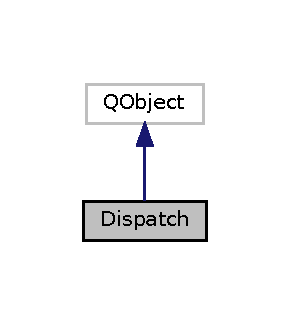
\includegraphics[width=139pt]{classDispatch__inherit__graph}
\end{center}
\end{figure}


Collaboration diagram for Dispatch\+:
\nopagebreak
\begin{figure}[H]
\begin{center}
\leavevmode
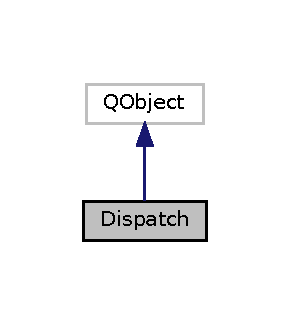
\includegraphics[width=139pt]{classDispatch__coll__graph}
\end{center}
\end{figure}
\subsection*{Public Slots}
\begin{DoxyCompactItemize}
\item 
\mbox{\Hypertarget{classDispatch_a1614e71f00049c8aa97656da43b9a760}\label{classDispatch_a1614e71f00049c8aa97656da43b9a760}} 
void {\bfseries turnout\+State\+Change} (Q\+String name)
\item 
\mbox{\Hypertarget{classDispatch_a1c92dd3797f9abd81064b81fa303f8bc}\label{classDispatch_a1c92dd3797f9abd81064b81fa303f8bc}} 
void {\bfseries message\+Received} (Q\+Json\+Document doc)
\item 
void \hyperlink{classDispatch_a9778159aee91f361533c1121b49b507b}{on\+Connected} ()
\end{DoxyCompactItemize}
\subsection*{Public Member Functions}
\begin{DoxyCompactItemize}
\item 
\mbox{\Hypertarget{classDispatch_aad7b6c1bd066e905cf3340061eed3edb}\label{classDispatch_aad7b6c1bd066e905cf3340061eed3edb}} 
{\bfseries Dispatch} (\hyperlink{classMessaging}{Messaging} $\ast$client)
\item 
void \hyperlink{classDispatch_aec3da26ad4b3550ce4d47fe5c5ed2f27}{add\+Turnout} (\hyperlink{classTurnout}{Turnout} $\ast$turnout, bool persist=true)
\begin{DoxyCompactList}\small\item\em Called when a turnout is added over M\+Q\+TT OR via the ini file. \end{DoxyCompactList}\end{DoxyCompactItemize}


\subsection{Detailed Description}
Provides dispatch type activities for handing messages received and send over time. Each new turnout is stored in a map, and when a message comes in for a specific turnout, that turnout is pulled from the map and acted on. 

\subsection{Member Function Documentation}
\mbox{\Hypertarget{classDispatch_aec3da26ad4b3550ce4d47fe5c5ed2f27}\label{classDispatch_aec3da26ad4b3550ce4d47fe5c5ed2f27}} 
\index{Dispatch@{Dispatch}!add\+Turnout@{add\+Turnout}}
\index{add\+Turnout@{add\+Turnout}!Dispatch@{Dispatch}}
\subsubsection{\texorpdfstring{add\+Turnout()}{addTurnout()}}
{\footnotesize\ttfamily void Dispatch\+::add\+Turnout (\begin{DoxyParamCaption}\item[{\hyperlink{classTurnout}{Turnout} $\ast$}]{turnout,  }\item[{bool}]{persist = {\ttfamily true} }\end{DoxyParamCaption})}



Called when a turnout is added over M\+Q\+TT OR via the ini file. 


\begin{DoxyParams}{Parameters}
{\em turnout} & A pointer to a \hyperlink{classTurnout}{Turnout} base which can ben L\+E\+F\+T/\+R\+I\+G\+H\+T/\+W\+YE \\
\hline
{\em persist} & Boolean which indicates whether we should try to persist this value\\
\hline
\end{DoxyParams}
This will take a new turnout pointer, send a notice over M\+Q\+TT that it was added and then store it to disk if that\textquotesingle{}s asked for via persist. \mbox{\Hypertarget{classDispatch_a9778159aee91f361533c1121b49b507b}\label{classDispatch_a9778159aee91f361533c1121b49b507b}} 
\index{Dispatch@{Dispatch}!on\+Connected@{on\+Connected}}
\index{on\+Connected@{on\+Connected}!Dispatch@{Dispatch}}
\subsubsection{\texorpdfstring{on\+Connected}{onConnected}}
{\footnotesize\ttfamily void Dispatch\+::on\+Connected (\begin{DoxyParamCaption}{ }\end{DoxyParamCaption})\hspace{0.3cm}{\ttfamily [slot]}}

Called async whenever the M\+Q\+TT client connects or reconnects 

The documentation for this class was generated from the following files\+:\begin{DoxyCompactItemize}
\item 
/home/pi/mrr\+\_\+turnouts/src/dispatch.\+h\item 
/home/pi/mrr\+\_\+turnouts/src/dispatch.\+cpp\end{DoxyCompactItemize}

\hypertarget{classLeftTurnout}{}\section{Left\+Turnout Class Reference}
\label{classLeftTurnout}\index{Left\+Turnout@{Left\+Turnout}}


Inheritance diagram for Left\+Turnout\+:
\nopagebreak
\begin{figure}[H]
\begin{center}
\leavevmode
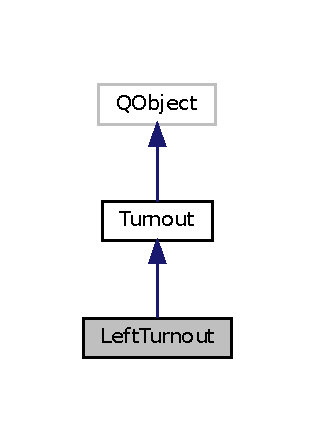
\includegraphics[width=151pt]{classLeftTurnout__inherit__graph}
\end{center}
\end{figure}


Collaboration diagram for Left\+Turnout\+:
\nopagebreak
\begin{figure}[H]
\begin{center}
\leavevmode
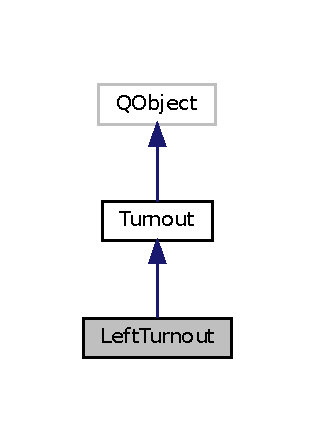
\includegraphics[width=151pt]{classLeftTurnout__coll__graph}
\end{center}
\end{figure}
\subsection*{Public Member Functions}
\begin{DoxyCompactItemize}
\item 
\mbox{\Hypertarget{classLeftTurnout_ae24ebadb9be727241ac5c4c4eb8b28cf}\label{classLeftTurnout_ae24ebadb9be727241ac5c4c4eb8b28cf}} 
{\bfseries Left\+Turnout} (int pin, Q\+String name)
\item 
\mbox{\Hypertarget{classLeftTurnout_a21a5aec6ff475925dc2b73cfb330b931}\label{classLeftTurnout_a21a5aec6ff475925dc2b73cfb330b931}} 
{\bfseries Left\+Turnout} (int pin)
\item 
\mbox{\Hypertarget{classLeftTurnout_a6a8de3619f56aa15e15bad2da854422c}\label{classLeftTurnout_a6a8de3619f56aa15e15bad2da854422c}} 
void {\bfseries switch\+Main} ()
\item 
\mbox{\Hypertarget{classLeftTurnout_ac8538da3d201212a772689c10a428ccd}\label{classLeftTurnout_ac8538da3d201212a772689c10a428ccd}} 
void {\bfseries switch\+Siding} ()
\item 
\mbox{\Hypertarget{classLeftTurnout_a21039a96b6d6de81d80f320ee34d1032}\label{classLeftTurnout_a21039a96b6d6de81d80f320ee34d1032}} 
void {\bfseries set\+State} (State state) override
\end{DoxyCompactItemize}
\subsection*{Additional Inherited Members}


The documentation for this class was generated from the following files\+:\begin{DoxyCompactItemize}
\item 
/home/pi/mrr\+\_\+turnouts/src/leftturnout.\+h\item 
/home/pi/mrr\+\_\+turnouts/src/leftturnout.\+cpp\end{DoxyCompactItemize}

\hypertarget{classMessaging}{}\section{Messaging Class Reference}
\label{classMessaging}\index{Messaging@{Messaging}}


Inheritance diagram for Messaging\+:
\nopagebreak
\begin{figure}[H]
\begin{center}
\leavevmode
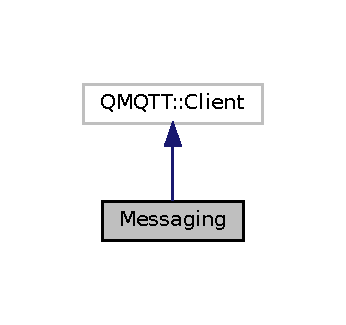
\includegraphics[width=166pt]{classMessaging__inherit__graph}
\end{center}
\end{figure}


Collaboration diagram for Messaging\+:
\nopagebreak
\begin{figure}[H]
\begin{center}
\leavevmode
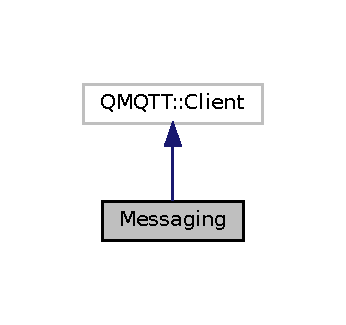
\includegraphics[width=166pt]{classMessaging__coll__graph}
\end{center}
\end{figure}
\subsection*{Public Slots}
\begin{DoxyCompactItemize}
\item 
\mbox{\Hypertarget{classMessaging_a227ca5e4baff6847a581e469859a3be9}\label{classMessaging_a227ca5e4baff6847a581e469859a3be9}} 
void {\bfseries on\+Connected} ()
\item 
\mbox{\Hypertarget{classMessaging_a482b88293ce9f86f2eaca43c3b71f27f}\label{classMessaging_a482b88293ce9f86f2eaca43c3b71f27f}} 
void {\bfseries on\+Disconnected} ()
\item 
\mbox{\Hypertarget{classMessaging_a298a8bcf6b1fa289d98508244c46c9ff}\label{classMessaging_a298a8bcf6b1fa289d98508244c46c9ff}} 
void {\bfseries on\+Received} (const Q\+M\+Q\+T\+T\+::\+Message \&message)
\item 
\mbox{\Hypertarget{classMessaging_a66df1b71b97968f743cca15a5ac5a858}\label{classMessaging_a66df1b71b97968f743cca15a5ac5a858}} 
void {\bfseries on\+Error} (const Q\+M\+Q\+T\+T\+::\+Client\+Error error)
\end{DoxyCompactItemize}
\subsection*{Signals}
\begin{DoxyCompactItemize}
\item 
\mbox{\Hypertarget{classMessaging_a0576dc58ba52f6dd1ca55e8a720c423b}\label{classMessaging_a0576dc58ba52f6dd1ca55e8a720c423b}} 
void {\bfseries client\+Connected} ()
\item 
\mbox{\Hypertarget{classMessaging_a2a96e2e73060387af9d5abc5d9eb71a4}\label{classMessaging_a2a96e2e73060387af9d5abc5d9eb71a4}} 
void {\bfseries message\+Received} (Q\+Json\+Document doc)
\end{DoxyCompactItemize}
\subsection*{Public Member Functions}
\begin{DoxyCompactItemize}
\item 
\mbox{\Hypertarget{classMessaging_a3b1df35f7818f802a808871d03462193}\label{classMessaging_a3b1df35f7818f802a808871d03462193}} 
{\bfseries Messaging} (const Q\+Host\+Address host, const quint16 port=1883, Q\+Object $\ast$parent=nullptr)
\end{DoxyCompactItemize}


The documentation for this class was generated from the following files\+:\begin{DoxyCompactItemize}
\item 
/home/pi/mrr\+\_\+turnouts/src/messaging.\+h\item 
/home/pi/mrr\+\_\+turnouts/src/messaging.\+cpp\end{DoxyCompactItemize}

\hypertarget{classRightTurnout}{}\section{Right\+Turnout Class Reference}
\label{classRightTurnout}\index{Right\+Turnout@{Right\+Turnout}}


Inheritance diagram for Right\+Turnout\+:
\nopagebreak
\begin{figure}[H]
\begin{center}
\leavevmode
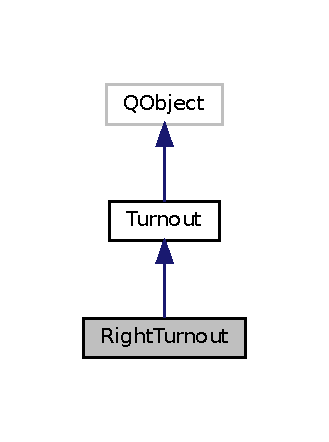
\includegraphics[width=158pt]{classRightTurnout__inherit__graph}
\end{center}
\end{figure}


Collaboration diagram for Right\+Turnout\+:
\nopagebreak
\begin{figure}[H]
\begin{center}
\leavevmode
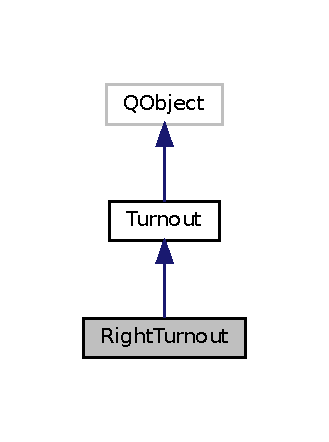
\includegraphics[width=158pt]{classRightTurnout__coll__graph}
\end{center}
\end{figure}
\subsection*{Public Member Functions}
\begin{DoxyCompactItemize}
\item 
\mbox{\Hypertarget{classRightTurnout_a8c48f203ce0d26584c5c7cb304bb9c3b}\label{classRightTurnout_a8c48f203ce0d26584c5c7cb304bb9c3b}} 
{\bfseries Right\+Turnout} (int pin, Q\+String name)
\item 
\mbox{\Hypertarget{classRightTurnout_a85d6bae3aebabe8df0179e44ea42ee6b}\label{classRightTurnout_a85d6bae3aebabe8df0179e44ea42ee6b}} 
{\bfseries Right\+Turnout} (int pin)
\item 
\mbox{\Hypertarget{classRightTurnout_a3240a6ed71c81faf116c05d0a45e5501}\label{classRightTurnout_a3240a6ed71c81faf116c05d0a45e5501}} 
void {\bfseries switch\+Main} ()
\item 
\mbox{\Hypertarget{classRightTurnout_a7e6fed6cad06da57209faf76035922e0}\label{classRightTurnout_a7e6fed6cad06da57209faf76035922e0}} 
void {\bfseries switch\+Siding} ()
\item 
\mbox{\Hypertarget{classRightTurnout_aad0a448c625a910706f4aa459b560127}\label{classRightTurnout_aad0a448c625a910706f4aa459b560127}} 
void {\bfseries set\+State} (State state) override
\end{DoxyCompactItemize}
\subsection*{Additional Inherited Members}


The documentation for this class was generated from the following files\+:\begin{DoxyCompactItemize}
\item 
/home/pi/mrr\+\_\+turnouts/src/rightturnout.\+h\item 
/home/pi/mrr\+\_\+turnouts/src/rightturnout.\+cpp\end{DoxyCompactItemize}

\hypertarget{classTurnout}{}\section{Turnout Class Reference}
\label{classTurnout}\index{Turnout@{Turnout}}


Inheritance diagram for Turnout\+:
\nopagebreak
\begin{figure}[H]
\begin{center}
\leavevmode
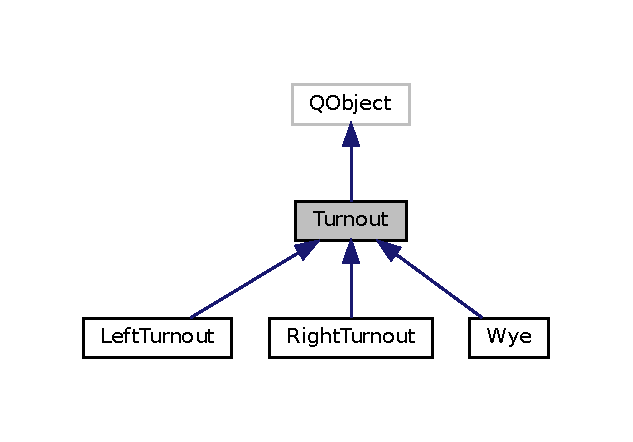
\includegraphics[width=304pt]{classTurnout__inherit__graph}
\end{center}
\end{figure}


Collaboration diagram for Turnout\+:
\nopagebreak
\begin{figure}[H]
\begin{center}
\leavevmode
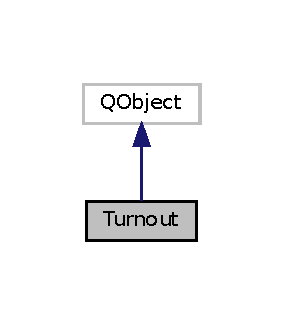
\includegraphics[width=136pt]{classTurnout__coll__graph}
\end{center}
\end{figure}
\subsection*{Public Types}
\begin{DoxyCompactItemize}
\item 
\mbox{\Hypertarget{classTurnout_aa7271edc7dd71de1993cb84efb433de4}\label{classTurnout_aa7271edc7dd71de1993cb84efb433de4}} 
enum {\bfseries Direction} \{ {\bfseries L\+E\+FT}, 
{\bfseries R\+I\+G\+HT}, 
{\bfseries W\+YE}
 \}
\item 
\mbox{\Hypertarget{classTurnout_a9b93fecdd78942538e79302c81fcc727}\label{classTurnout_a9b93fecdd78942538e79302c81fcc727}} 
enum {\bfseries State} \{ {\bfseries M\+A\+IN}, 
{\bfseries S\+I\+D\+I\+NG}
 \}
\end{DoxyCompactItemize}
\subsection*{Signals}
\begin{DoxyCompactItemize}
\item 
\mbox{\Hypertarget{classTurnout_af184ceca5457de620541017d711204b6}\label{classTurnout_af184ceca5457de620541017d711204b6}} 
void {\bfseries state\+Change} (Q\+String name)
\end{DoxyCompactItemize}
\subsection*{Public Member Functions}
\begin{DoxyCompactItemize}
\item 
\mbox{\Hypertarget{classTurnout_a5f5e6fc12ec957758010cd4eb3ed41b7}\label{classTurnout_a5f5e6fc12ec957758010cd4eb3ed41b7}} 
{\bfseries Q\+\_\+\+E\+N\+UM} (Direction)
\item 
\mbox{\Hypertarget{classTurnout_a337a41170c90bd67ce308c0a39be83ab}\label{classTurnout_a337a41170c90bd67ce308c0a39be83ab}} 
{\bfseries Turnout} (int pin, Q\+String name, Direction dir, Q\+Object $\ast$parent=nullptr)
\item 
\mbox{\Hypertarget{classTurnout_ad732b5d164b51989efbf15910e89207a}\label{classTurnout_ad732b5d164b51989efbf15910e89207a}} 
{\bfseries Turnout} (int pin, Direction dir, Q\+Object $\ast$parent=nullptr)
\item 
\mbox{\Hypertarget{classTurnout_a3756614bdf1954b7855a29148bc388e6}\label{classTurnout_a3756614bdf1954b7855a29148bc388e6}} 
void {\bfseries no} ()
\item 
\mbox{\Hypertarget{classTurnout_ad012bbace4a365d530640c511b69014f}\label{classTurnout_ad012bbace4a365d530640c511b69014f}} 
void {\bfseries nc} ()
\item 
\mbox{\Hypertarget{classTurnout_a18d8e29c202ed64091fcc9c61c06cbaf}\label{classTurnout_a18d8e29c202ed64091fcc9c61c06cbaf}} 
Q\+String {\bfseries name} ()
\item 
\mbox{\Hypertarget{classTurnout_ae2f2d2c69fe1cc863b29064092460c62}\label{classTurnout_ae2f2d2c69fe1cc863b29064092460c62}} 
Q\+String {\bfseries direction} ()
\item 
\mbox{\Hypertarget{classTurnout_a1f27c3cd43df36267f9311fc4fbd58fb}\label{classTurnout_a1f27c3cd43df36267f9311fc4fbd58fb}} 
Q\+String {\bfseries state} ()
\item 
\mbox{\Hypertarget{classTurnout_a276a6d7779e7191057adc89c35cf7333}\label{classTurnout_a276a6d7779e7191057adc89c35cf7333}} 
int {\bfseries pin} ()
\item 
\mbox{\Hypertarget{classTurnout_ae7197fb76f53d720c0fa2828746bd913}\label{classTurnout_ae7197fb76f53d720c0fa2828746bd913}} 
virtual bool {\bfseries is\+On\+Main} ()
\item 
\mbox{\Hypertarget{classTurnout_a0f99553ab7a67b90e449bf22f7594d8e}\label{classTurnout_a0f99553ab7a67b90e449bf22f7594d8e}} 
virtual void {\bfseries set\+State} (State state)=0
\end{DoxyCompactItemize}
\subsection*{Protected Attributes}
\begin{DoxyCompactItemize}
\item 
\mbox{\Hypertarget{classTurnout_a0e975ccac37e52ad1cad7adea5ef130b}\label{classTurnout_a0e975ccac37e52ad1cad7adea5ef130b}} 
Direction {\bfseries m\+\_\+direction}
\item 
\mbox{\Hypertarget{classTurnout_a86db8a9921b41043a984efbeada6d861}\label{classTurnout_a86db8a9921b41043a984efbeada6d861}} 
int {\bfseries m\+\_\+pin}
\item 
\mbox{\Hypertarget{classTurnout_aeb7d7a0b3f175d60f07babe7b6173988}\label{classTurnout_aeb7d7a0b3f175d60f07babe7b6173988}} 
Q\+String {\bfseries m\+\_\+name}
\item 
\mbox{\Hypertarget{classTurnout_ab4e32db640be95dbd4c0d7ca70a43b45}\label{classTurnout_ab4e32db640be95dbd4c0d7ca70a43b45}} 
State {\bfseries m\+\_\+state}
\end{DoxyCompactItemize}


The documentation for this class was generated from the following files\+:\begin{DoxyCompactItemize}
\item 
/home/pi/mrr\+\_\+turnouts/src/turnout.\+h\item 
/home/pi/mrr\+\_\+turnouts/src/turnout.\+cpp\end{DoxyCompactItemize}

\hypertarget{classWye}{}\section{Wye Class Reference}
\label{classWye}\index{Wye@{Wye}}


Inheritance diagram for Wye\+:
\nopagebreak
\begin{figure}[H]
\begin{center}
\leavevmode
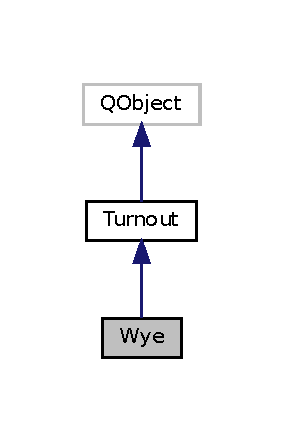
\includegraphics[width=136pt]{classWye__inherit__graph}
\end{center}
\end{figure}


Collaboration diagram for Wye\+:
\nopagebreak
\begin{figure}[H]
\begin{center}
\leavevmode
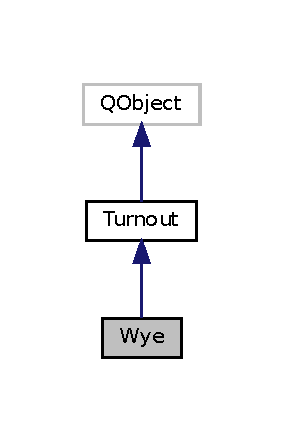
\includegraphics[width=136pt]{classWye__coll__graph}
\end{center}
\end{figure}
\subsection*{Public Member Functions}
\begin{DoxyCompactItemize}
\item 
\mbox{\Hypertarget{classWye_a3e77a490a8ed9769ae614ed6c0b5120d}\label{classWye_a3e77a490a8ed9769ae614ed6c0b5120d}} 
{\bfseries Wye} (int pin, Q\+String name)
\item 
\mbox{\Hypertarget{classWye_ad9b9aec2c48aaf06f000bf1777ec8e02}\label{classWye_ad9b9aec2c48aaf06f000bf1777ec8e02}} 
{\bfseries Wye} (int pin)
\item 
\mbox{\Hypertarget{classWye_ad6d6484f6e9fc7076ca8974eb32d7a64}\label{classWye_ad6d6484f6e9fc7076ca8974eb32d7a64}} 
void {\bfseries switch\+Main} ()
\item 
\mbox{\Hypertarget{classWye_ac74866da6e73a1f1c692dbdeea6804be}\label{classWye_ac74866da6e73a1f1c692dbdeea6804be}} 
void {\bfseries switch\+Siding} ()
\item 
\mbox{\Hypertarget{classWye_a2a0551f36af31b003502f0ce976f0044}\label{classWye_a2a0551f36af31b003502f0ce976f0044}} 
void {\bfseries set\+State} (State state)
\end{DoxyCompactItemize}
\subsection*{Additional Inherited Members}


The documentation for this class was generated from the following files\+:\begin{DoxyCompactItemize}
\item 
/home/pi/mrr\+\_\+turnouts/src/wye.\+h\item 
/home/pi/mrr\+\_\+turnouts/src/wye.\+cpp\end{DoxyCompactItemize}

%--- End generated contents ---

% Index
\backmatter
\newpage
\phantomsection
\clearemptydoublepage
\addcontentsline{toc}{chapter}{Index}
\printindex

\end{document}
